\section{Мета практикуму}
Практично ознайомитися із тестами перевірки чисел на простоту, методами генерації ключів для асиметричної криптосистеми типу RSA, протоколом розсилання ключів та безпосередньо реалізувати їх.

\subsection{Постановка задачі та варіант}
\begin{tabularx}{\textwidth}{X|X}
	\textbf{Треба реалізувати} & \textbf{Зроблено} \\
	PRNG & DefaultPRNG \checkmark\\
	Miller-Rabin test & \checkmark\\
	Extended Euclidian algorithm & \checkmark\\ 
	RSA Encrypt/Decrypt & \checkmark\\
	RSA Sign/Verify  & \checkmark\\
	RSA Send/Receive  key & \checkmark\\
\end{tabularx}
\end{center}


\section{Хід роботи/Опис труднощів}
На початку релазіції практикуму, треба було вибрати генератор псевдовипадкових чисел із попередньої лабораторної роботи та  використати тут. Не довго думаючи, обрав влаштований генератор, що працює на алгоритмі ChaCha12 і дає найкращі результати на тестуванні послідовності. Труднощів із реалізацією самої криптосистеми RSA не було, одразу  функціонал підпису та шифрування розбив на RsaEncryptor, RsaSigner, що спростило подальшу роботу. Також проблем із написанням тесту Міллера-Рабіна, розширеного алгоритму Евкліда не виникало, адже вони уже були написані і відлагоджені у курсі Теоретико-Числових Алгортимів.
Хочу додати, що для генерації простого числа застосовую комбінацію алгоритмів Міллера-Рабіна та пробні ділення (перші 100 простих). Уже для 2048 бітних чисел треба куди більше часу чекати, ніж на менші, але дочекатися можна. 

Основна проблема була із перевіркою вихідних даних із сервером та із протоколом обміну ключем між користувачами. Головне, що я упустив, що функції: 
\begin{enumerate}
	\item  SendKey() --- спочатку записуємо собі публічний ключ сервера, потім зашифровуємо ключ та надіслаємо підписану пару назад (кроки 0, 1);
	\item ReceiveKey() --- надаємо свій публічний ключ, де сервер у свою чергу зашифрує повідомлення та надсилає нам (кроки 2,3).
\end{enumerate}

\begin{remark}
	 Нульовим кроком вважаю надсилання публічного ключа користувача $B>A$.
\end{remark}


\begin{figure}[h]
			\center{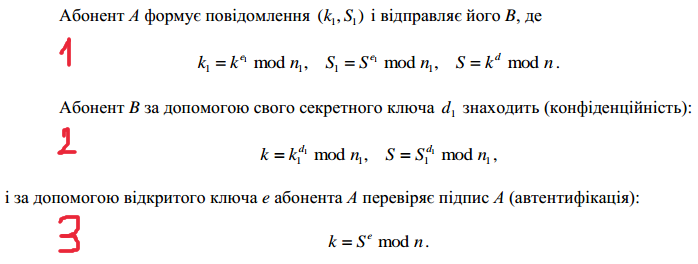
\includegraphics[scale = 0.47]{key_exchange}}
			\caption{Вигляд протоколу.}
			\label{fig:protocole}
		\end{figure}

\newpage


\section{Результати дослідження}
%Результати тестування чисел на простоту наведені у наступній таблиці.

\begin{table}
\begin{tabularx}{\textwidth}{c|c|c}

\textbf{$\#$ біт} & Число у HEX & Просте?\\
	$256$ & \substack{ $0xDA44D604C658EAA955379B1B7B94F321$\\ $B6A690462AA14483A0C387A1E0D362D9$}& $false$
	\\[2em] 
	$256$ & \substack{ $0xDBF6CB5A81388144448A6387CC960642$\\ $5551B6A6833B30E1C736CFEE4FD98F33$}& $false$
	\\[2em] 
	$256$ & \substack{ $0x3393DFF87DC8C9FAA2C8C31597BB3C66$\\ $076BF4CBC331E38F9679D368F6746239$}& $true$
	\\[2em] 
	$256$ & \substack{ $0x17CCA6C243E91E490147765C97BD3F7D$\\ $42E5FE4C21F2C6F878337BA30C889007$}& $true$
	\\[2em] 
	$128$ & \substack{ $0x4203E2FF7902D5725FE064183FC35681$ } & $false$
	\\[2em] 
	$128$ & \substack{ $0xD705D142F93F21868CBBA75E5B06388$ }& $false$
	\\[2em]
	$128$ & \substack{ $0xE3856FDE94235F7457F7B023BD918D6D$ }& $true$
	\\[2em] 
	$128$ & \substack{ $0xFB23844228242601CEE61AEE41E66525$ }& $true$
	\\[2em] 
	\end{tabularx}
	      \caption{Результати тестування чисел на простоту алгортимом Міллера-Рабіна}
\end{table}


Наведу числені результати виконання програми для ключів 128 та 256 біт.

\begin{table}
\begin{tabularx}{\textwidth}{c|c|c}

\textbf{$\#$ біт} & n  &  e\\
	$128$ & \substack{ $883CEC2DC61C496CC99199CC1C9416E5$}& \substack{ $10001$}
	\\[2em] 
	$256$ & \substack{ $8C9AE8DD1243B91B291034D99C4B2C6E$\\ $9141D8B2E0B3F255E1B60AA6473014B7$}& \substack{ $10001$}
	\\[2em] 
	\end{tabularx}
	      \caption{Публічні ключі 1,2.}
\end{table}

\begin{table}
\begin{tabularx}{\textwidth}{c|c|c|c}

\textbf{$\#$ біт} & \textbf{Особистий ключ №1} & \textbf{$\#$ біт} & \textbf{Особистий ключ №2} \\
	$128$ & \substack{ $n = 15df8f40346b5b3441655b57380fb7eb$ } & $256$ & \substack{ $n = 91fbf48e2e7324ef16f0faa145a41625$ & $f2e06886b5c4f461bf6fd513e9fd799b$ } 
	\\[2em] 
	$-$ & \substack{ $e = 10001 $} & $-$ & \substack{ $e = 10001 $}
	\\[2em] 
	$-$ & \substack{ $d = c6b700f68b43c88a2eb58b3d3edce01$} & $-$ & \substack{ $d = 3bfb7a90b1253e97bea56555be779d61$ & $7822a9d70be57c2d03b528fd02378681$}
	\\[2em] 
	$-$ & \substack{ $primes = [c5c22fa2cc1c442b,$ & $1c50aca1dec5bb41]$} & $-$ & \substack{ $primes = [ed5198a17488705858bb68d817e5175f,$ & $9d79cd5e9562c54492a4c974c151f345]$}
	\\[2em] 
	\end{tabularx}
	      \caption{Особисті ключі 1,2.}
\end{table}

\begin{remark}
	Повідомленням за замовчуванням вважаю --- $ABCDEF123456789$.
\end{remark}

\begin{example}
\end{example}

\begin{enumerate}
\item
	\begin{enumerate}
		\item Шифруємо повідомлення публічним ключем №1: $66F4C31219CC070D2725B4EB9D34913D$,
		\item Розшифровка сервера повідомлення: $0ABCDEF123456789$.
	\end{enumerate}

\item
	\begin{enumerate}
		\item Сервер шифрує повідомлення приватним ключем №2:$\substack{ $17D126D38F6FA437130F625C61FC593$\\ $7772BEC1B732E46DF0D6BE92E470CFFAD$}$,
		\item Розшифровуємо попереднє повідомлення приватним ключем №2: $ABCDEF123456789$.
	\end{enumerate}
	
\item 
	\begin{enumerate}
		\item Підписуємо повідомлення приватним ключем №2: 
		
		\begin{enumerate}		
			\item $\substack{ $s = 57B7156804546A4DD2EB54C9490655EA$\\ $6B87AFEFE754B0F5F810BF70D996B2C3$}$,
		 	\item $m = ABCDEF123456789$, 
		 	\item $is$-$ok=true$.
		 \end{enumerate}
		\item Підписуємо повідомлення приватним ключем №1: 
		\begin{enumerate}	
			\item $s=5D1BEC41053A2C59035AFA74E951B92$, 
			\item $m=0xABCDEF123456789$, 
			\item $is$-$ok=true$.
		\end{enumerate}
	\end{enumerate}
\end{enumerate}


\begin{table}
\begin{tabularx}{\textwidth}{c|c|c}

\textbf{Напрям} & \textbf{Дані} \\
	$A>B$ & \substack{ $n=91fbf48e2e7324ef16f0faa145a41625$ & $f2e06886b5c4f461bf6fd513e9fd799b$ } & \substack{ $e=10001$}
	\\[2em] 
	$A<B$ & \substack{ $key = 55FA139F08277E93FB22A5D9E730965C$ & $C0F2140644D0249AD7AC64DBEE18A9DA$}& \substack{ $s = 19B568288BB4C6442243BD535FFE8A72$ & $85B65BB5016169DCA77AB2E049219B38$}
	\\[2em] 
	$A$ & \substack{ $key = C189A5C812E05395$}& \substack{ $is$_$ok = true$}
	\\[2em] 
	\end{tabularx}
	      \caption{ Приклад дешифрування по протоколу 1 (Публічний ключ №1, особистий ключ №2).}
\end{table}

\begin{table}
\begin{tabularx}{\textwidth}{c|c|c}

\textbf{Напрям} & \textbf{Дані} \\
	$A<B$ &  \substack{ $n=8C9AE8DD1243B91B291034D99C4B2C6E$ & $9141D8B2E0B3F255E1B60AA6473014B7$ } & \substack{ $e=10001$}
	\\[2em] 
	$A>B$ & \substack{ $key = 5263AEF93A9B9DA25F66A66276CF9FCC$ & $FD2ADE9A72488ECA3567DB1B7B942D11$}& \substack{ $s = 14418308DAA7CEA590A693591BFF8FED$ & $4B6CB0C3ECD7B6D492D1D72D9950BDDC$}
	\\[2em] 
	$B$ & \substack{ $key = ABCDEF123456789$}& \substack{ $is_ok = true$}
	\\[2em] 
	\end{tabularx}
	      \caption{ Приклад надсилання ключа (Публічний ключ №2, особистий ключ №1).}
\end{table}

\begin{figure}[h]
			\center{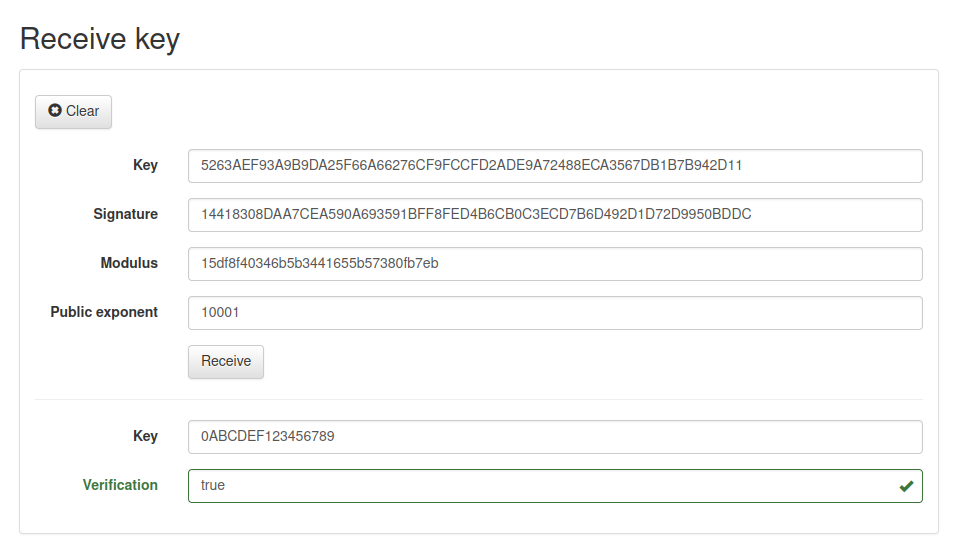
\includegraphics[scale = 0.4]{key_exchange_result}}
			\caption{Результат надсилання ключа №2.}
			\label{fig:image}
		\end{figure}

\begin{remark}
Інші приклади шифрування, підпису на більших числах є у файлі додатку до звіту --- <<appendix\textunderscore to\textunderscore report.txt>> .
\end{remark}


Із вище зазначених результатів дослідження можна зробити висновок, що:
\begin{itemize}
\item Умову $n_1 \geq n$ у протоколі передачі ключа треба виконувати обов'язково, адже за іншої умови будемо отримувати неправильні повідомлення. Доприкладу, візьмемо (100 mod 10) mod 49, вийде неправильна відповідь, коли треба брати $100$ mod $49$;
\item Криптосистема напряму залежна від простоти чисел, довжини n та інших критеріїв, що при невиконанні усіх умов буде давати ніяк незахищене з'єднання.
\end{itemize}

\section{Висновки}
За допомогою реалізації практикуму ''Вивчення криптосистеми RSA та алгоритму електронного
підпису'' дізнався на практиці, як генеруться параметри для асиметричних криптосистем та як реалізовувати їх. 

Рекомендую для алгоритмів знаходження псевдопростих чисел одразу додавати алгоритм пробних ділень. Він значно скоротить час перебору чисел.

		

	




